\documentclass[11pt]{beamer}
\usetheme{Warsaw}
\usepackage[utf8]{inputenc}
\usepackage[french]{babel}
\usepackage[T1]{fontenc}
\usepackage{amsmath}
\usepackage{amsfonts}
\usepackage{amssymb}
\usepackage{graphicx}
%%\usepackage[utf8x]{inputenc}
\usepackage[T1]{fontenc}
\usepackage{lmodern}

\usepackage{ifthen}
\usepackage{url}


\usepackage{multirow}

% Color
% cfr http://en.wikibooks.org/wiki/LaTeX/Colors
\usepackage{color}
\usepackage[usenames,dvipsnames,svgnames,table]{xcolor}
\definecolor{dkgreen}{rgb}{0.25,0.7,0.35}
\definecolor{dkred}{rgb}{0.7,0,0}

\newcommand{\matlab}{\textsc{Matlab}}

% Math symbols
\usepackage{amsmath}
\usepackage{amssymb}
\usepackage{amsthm}
\DeclareMathOperator*{\argmin}{arg\,min}
\DeclareMathOperator*{\argmax}{arg\,max}


% Sets
\newcommand{\Z}{\mathbb{Z}}
\newcommand{\R}{\mathbb{R}}
\newcommand{\Rn}{\R^n}
\newcommand{\Rnn}{\R^{n \times n}}
\newcommand{\C}{\mathbb{C}}
\newcommand{\K}{\mathbb{K}}
\newcommand{\Kn}{\K^n}
\newcommand{\Knn}{\K^{n \times n}}

% Unit vectors
\usepackage{esint}
\usepackage{esvect}
\newcommand{\kmath}{k}
\newcommand{\xunit}{\hat{\imath}}
\newcommand{\yunit}{\hat{\jmath}}
\newcommand{\zunit}{\hat{\kmath}}
\newcommand{\uunit}{\hat{\umath}}

% rot & div & grad & lap
\DeclareMathOperator{\newdiv}{div}
\newcommand{\divn}[1]{\nabla \cdot #1}
\newcommand{\rotn}[1]{\nabla \times #1}
\newcommand{\grad}[1]{\nabla #1}
\newcommand{\gradn}[1]{\nabla #1}
\newcommand{\lap}[1]{\nabla^2 #1}


% Elec
\newcommand{\B}{\vec B}
\newcommand{\E}{\vec E}
\newcommand{\EMF}{\mathcal{E}}
\newcommand{\perm}{\varepsilon} % permittivity

\newcommand{\bigoh}{\mathcal{O}}
\newcommand\eqdef{\triangleq}

\DeclareMathOperator{\newdiff}{d} % use \dif instead
\newcommand{\dif}{\newdiff\!}
\newcommand{\fpart}[2]{\frac{\partial #1}{\partial #2}}
\newcommand{\ffpart}[2]{\frac{\partial^2 #1}{\partial #2^2}}
\newcommand{\fdpart}[3]{\frac{\partial^2 #1}{\partial #2\partial #3}}
\newcommand{\fdif}[2]{\frac{\dif #1}{\dif #2}}
\newcommand{\ffdif}[2]{\frac{\dif^2 #1}{\dif #2^2}}
\newcommand{\constant}{\ensuremath{\mathrm{cst}}}

\usepackage{siunitx}

\usepackage{tikz}

\usepackage{pgfplots}
\usepackage{lmodern}
\usepackage{microtype}
\usepackage{xspace}

\usepackage{babel}
% Listing
% always put it after babel
% http://tex.stackexchange.com/questions/100717/code-in-lstlisting-breaks-document-compile-error
\usepackage{listings}

\definecolor{mygreen}{rgb}{0,0.6,0}
\definecolor{mygray}{rgb}{0.5,0.5,0.5}
\definecolor{mymauve}{rgb}{0.58,0,0.82}
\lstset{ %
  language=Matlab,
  backgroundcolor=\color{white},   % choose the background color; you must add \usepackage{color} or \usepackage{xcolor}
  basicstyle=\footnotesize,        % the size of the fonts that are used for the code
  breakatwhitespace=false,         % sets if automatic breaks should only happen at whitespace
  breaklines=true,                 % sets automatic line breaking
  captionpos=b,                    % sets the caption-position to bottom
  commentstyle=\color{mygreen},    % comment style
  deletekeywords={...},            % if you want to delete keywords from the given language
  escapeinside={\%*}{*)},          % if you want to add LaTeX within your code
  extendedchars=true,              % lets you use non-ASCII characters; for 8-bits encodings only, does not work with UTF-8
  frame=single,	                   % adds a frame around the code
  keepspaces=true,                 % keeps spaces in text, useful for keeping indentation of code (possibly needs columns=flexible)
  keywordstyle=\color{blue},       % keyword style
  otherkeywords={*,...},           % if you want to add more keywords to the set
  numbers=none,                    % where to put the line-numbers; possible values are (none, left, right)
  numbersep=5pt,                   % how far the line-numbers are from the code
  numberstyle=\tiny\color{mygray}, % the style that is used for the line-numbers
  rulecolor=\color{black},         % if not set, the frame-color may be changed on line-breaks within not-black text (e.g. comments (green here))
  showspaces=false,                % show spaces everywhere adding particular underscores; it overrides 'showstringspaces'
  showstringspaces=false,          % underline spaces within strings only
  showtabs=false,                  % show tabs within strings adding particular underscores
  stepnumber=2,                    % the step between two line-numbers. If it's 1, each line will be numbered
  stringstyle=\color{mymauve},     % string literal style
  tabsize=2,	                   % sets default tabsize to 2 spaces
  title=\lstname                   % show the filename of files included with \lstinputlisting; also try caption instead of title
}

\KOMAoptions{DIV=last}

\usepackage[top = 2.5 cm, bottom = 3 cm, left = 2.5 cm, right = 2.5 cm]{geometry}
\usepackage{caption}

\title{LELEC2103 - Projet 3 in Electricity}
\subtitle[\ldots]{Result of the lab 3 and lab 4}
\author[D. Deprez\and B. Ouachalih]{Damien Deprez\and Bilal Ouachalih}
\institute{EPL}
\date{28th october 2016}

\begin{document}

% TITLE PAGE
{
	\setbeamertemplate{headline}{}  
	\setbeamertemplate{footline}{}
	\setbeamertemplate{navigation symbols}{}
	\begin{frame}[noframenumbering]
		\titlepage
	\end{frame}
} 

% TABLE OF CONTENTS
{
	\setbeamertemplate{navigation symbols}{}
	\setbeamertemplate{headline}{}
	\begin{frame}[noframenumbering]{Plan de la présentation}
		\tableofcontents
	\end{frame}
}

\section{Symbol timing recovery}

\subsection{Maximum Energy}
\subsubsection{Direct Maximum Energy}
\begin{frame}
\frametitle{}

Channel canal

\begin{equation}
z(t)=\alpha\exp^{j\phi} x(t-\tau_{d})+v(t)
\label{equ1}
\end{equation}

\begin{itemize}

\item Direct maximisation of the output energy
\begin{equation}
J_{approx}[k] = \frac{1}{P} \sum \limits_{p=0}^{P-1} |r(pT+\frac{kT}{M})|^2
\label{equ1}
\end{equation}


\end{itemize}

\end{frame}

\subsubsection{Earlygate}

\begin{frame}

Indirect maximisation of the output energy
\begin{equation}
\hat{k}= {arg\min}_{k=0,..,M-1} J_{\delta}[k]
\end{equation}

\end{frame}

\subsection{Result}
\subsubsection{Timing Static Error}
\begin{frame}
\frametitle{Timing Static error VS RX Oversampling factor}
\begin{figure}
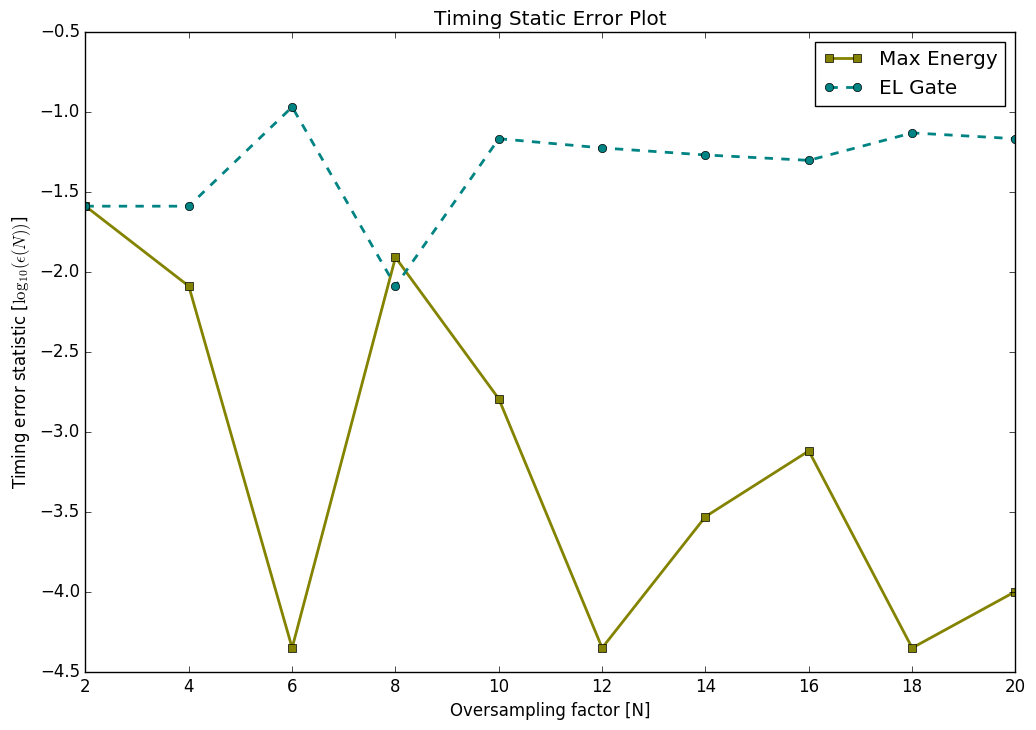
\includegraphics[width=0.9\textwidth]{img/Timing-Static-Error.png}
\end{figure}

\end{frame}

\subsubsection{Constellation}

\begin{frame}
\frametitle{Impact of the oversampling factor at the receiver}

\begin{figure}
   \begin{minipage}[c]{.46\linewidth}
   \centering
   {\large Constellation for N=2}
            \tiny
      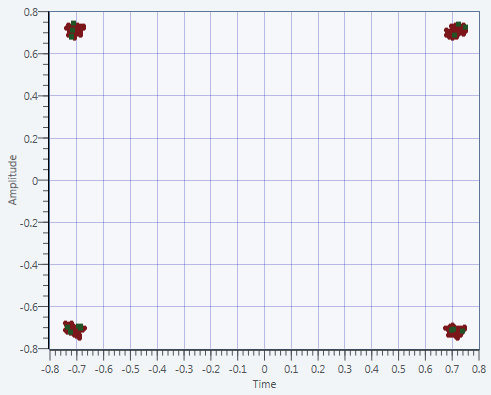
\includegraphics[width=1\textwidth]{img/ConstellationN2-MaxEnergy.png}
      
   \end{minipage} \hfill
   \begin{minipage}[c]{.46\linewidth}
   \centering
   {\large Constellation for N=20}
            \tiny
      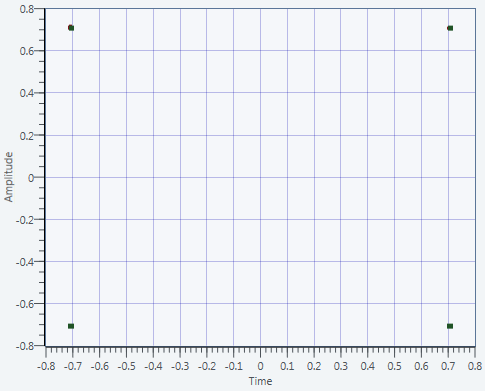
\includegraphics[width=1\textwidth]{img/ConstellationN20-MaxEnergy.png}
   \end{minipage}
\end{figure}

\end{frame}
\begin{frame}
\frametitle{Effect of M on the Max Energy method}

\begin{itemize}

\item If M is increasing => Result at the receiver  is better. Why ?

\item In equation \ref{equ1}, if M is incresing, 



\end{itemize}



\end{frame}

\section{Channel Estimation and Equalization}
\subsection{Purpose of the lab}
\begin{frame}
Channel canal
\begin{equation}
z(t) = \alpha_0 e^{j\phi_0}x(t-\tau_0) + \alpha_1 e^{j\phi_1}x(t-\tau_1) + v(t)
\end{equation}
Direct Least-Squares Equalizer
\begin{equation}
t[n] = \sum_{l=0}^{L_f} {f_{n_d}[l]y[n + n_d -l ]}
\end{equation}
\end{frame}
\subsection{Result}
\subsubsection{Effect of the equalizer length}
\begin{frame}
\frametitle{Impact of the equlizer length at the reciever}
\begin{minipage}[c]{0.46\linewidth}
\centering 
{Constellation for $L_f + 1 = 2$}
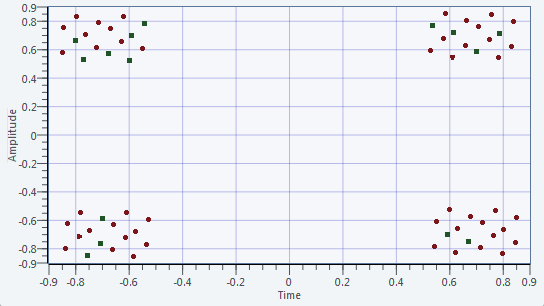
\includegraphics[width=\textwidth]{img/ISI-2}
\end{minipage}
\begin{minipage}[c]{0.46\linewidth}
\centering 
{Constellation for $L_f + 1 = 6$}
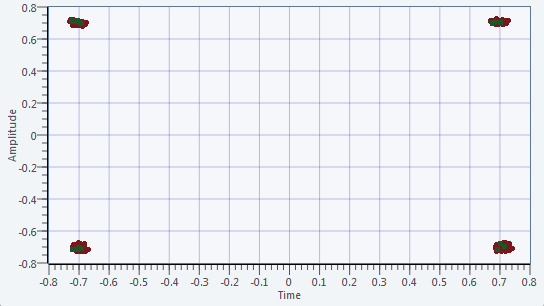
\includegraphics[width=\textwidth]{img/ISI-6}
\end{minipage}
\end{frame}
\subsubsection{Effect of the noise}
\begin{frame}
\frametitle{Impact of the noise at the reciever}
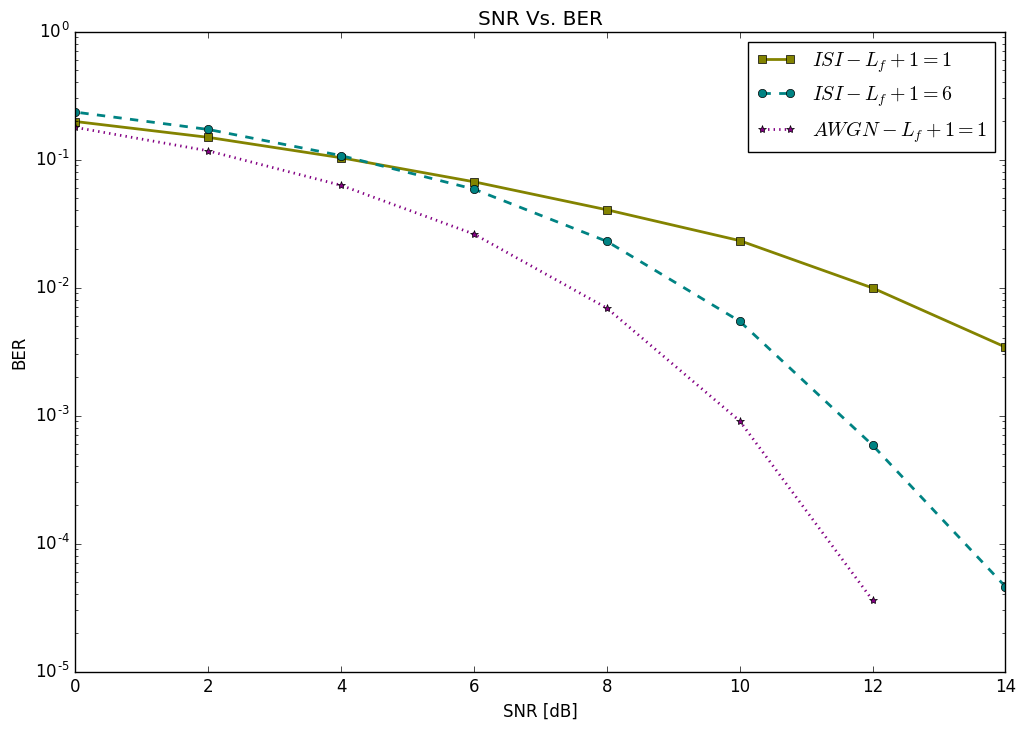
\includegraphics[width=.9\linewidth]{img/SNR}
\end{frame}
\subsubsection{Experiment on the USRP}
\begin{frame}
\frametitle{Experiment on the USRP}
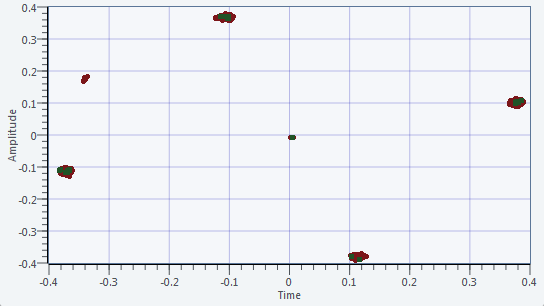
\includegraphics[width=.9\linewidth]{img/USRP-Rotate}
\end{frame}

\end{document}